\documentclass{article}
\usepackage[utf8]{inputenc}
\usepackage[T1]{fontenc} % ASCII-friendly formatting of text
\usepackage{parskip} % no indentation of paragraphs
\usepackage{courier} % for use in lstlistings
\usepackage[margin=1in]{geometry}

\usepackage{titlesec} % for making sub-subsections
\setcounter{secnumdepth}{3}

\usepackage{float} % for manipulating floats like tables and figures
\restylefloat{table} % allows you to use "H" for hard-fixing table position
\usepackage{graphicx} % for including figures

\usepackage{csquotes} % for block quotes

\usepackage{hyperref}
\newcommand\fnurl[2]{%
  \href{#2}{#1}\footnote{\url{#2}}%
} %for putting hyperlinks in footnotes

\usepackage{listings} % include source code
\usepackage{color} % color source code

\newcommand{\pltlang}{d.o.t.s.} % allows us to just reference the language name with the ``\pltlang'' cmd, so we can change the name later w/o too much hassle

\newcommand{\code}[1]{\texttt{#1}} %sets it up so you can use \code{...} to format text

\definecolor{codegreen}{rgb}{0,0.6,0}
\definecolor{codegray}{rgb}{0.5,0.5,0.5}
\definecolor{codebrown}{rgb}{0.7,0.35,0.25}
\definecolor{backcolor}{rgb}{0.95,0.95,0.92}

\lstdefinestyle{pltStyle}{
  basicstyle=\ttfamily,
  backgroundcolor=\color{backcolor},
  commentstyle=\color{codebrown},
  keywordstyle=\color{blue},
  numberstyle=\tiny\color{codegray},
  stringstyle=\color{codegreen},
  breakatwhitespace=false,
  breaklines=true,
  captionpos=b,
  keepspaces=false,
  numbers=left,
  numbersep=5pt,
  showspaces=false,
  showstringspaces=false,
  showtabs=false,
  tabsize=2
}

\lstdefinelanguage{pltLang}
{
  morekeywords={
    bool,
    true,
    false,
    num,
    string,
    null,
    INF,
    if,
    else,
    for,
    while,
    break,
    in,
    node,
    graph,
    list,
    dict,
    print,
    range,
    def,
    return
  },
  sensitive=true, %keywords are case sensitive
  morecomment=[l]{\#}, % symbol for single-line comment
  morecomment=[s]{\\*}{*\\}, % symbol for multi-line comment
  morestring=[b]" % sets double quote as string indicator
}

\lstset{style=pltStyle, columns=flexible}

\title{d.o.t.s. \\ A graph language.}
\author{Hosanna Fuller (hjf2106) --- Manager\\
Rachel Gordon (rcg2130) --- Language Guru\\
Yumeng Liao (yl2908) --- Tester\\
Adam Incera (aji2112) --- System Architect}
\date{September 2015}

\begin{document}

\maketitle

\tableofcontents
\newpage

\section{Lexical Elements}

\subsection {Whitespace}
In \pltlang\, white space is defined as any of the special characters \code{\textbackslash r\textbackslash n}, \code{\textbackslash n},  and \code{\textbackslash t} as well as the character obtained by pressing the spacebar. The space character sometimes delimits a separation between the parts of an expression (see the rest of the manual for syntax specifics), but otherwise whitespace is generally ignored outside of string and char expressions, as expressions are separated by the semicolon and scope is defined by braces. 


\section{Data Types}

\subsection{Primitive Types}

\subsubsection{num}

The \code{num} data type represents all numbers in \pltlang\ There is no distinction between the traditional data types of \code{int} and \code{float}, which means for example that there is no difference between the values \code{5} and \code{5.0}. The comparative ordering of nums is the same as that of numbers in mathematics. 

\begin{lstlisting}[language=pltLang, caption=Declaration of ``num'' types., label=lst:num]
num x = 5;
num y = 5.0;
num z = x;

num q = 3.14159;

num a, b, c;
\end{lstlisting}

In Listing \ref{lst:num} variables \code{a, b, c, x, y, z}, and \code{q} are all of the type \code{num}. Variables \code{x}, \code{y}, and \code{z} store equivalent values. Variables \code{a}, \code{b}, and \code{c} are all equal to \code{null}.

\subsubsection{string}

A \code{string} is a sequence of 0 or more characters. Comparative ordering of strings is determined sequentially by comparing the ASCII value of each character in the two strings from left to right.

\begin{lstlisting}[language=pltLang, caption=Declaration of ``string'' types., label=lst:string]
string a = "alpha";
string empty = "";
string char = "a";
\end{lstlisting}

\subsubsection{bool}

The \code{bool} type is a logical value which can be either the primitive values \code{true} or \code{false}.

\begin{lstlisting}[language=pltLang, caption=Declaration of ``bool'' types., label=lst:bool]
bool t = true;
bool f = false;
\end{lstlisting}

\section{Expressions and Operators}

\subsection{Node Operators}

The node operators outlined in Table \ref{tbl:node-ops} below are all binary operators which take a node object on the left-hand and right-hand sides of the operator.

\begin{table}[H]
\centering
\begin{tabular}{| p{1.5in} | p{2.75in} |}
\hline
Operator & Explanation \\
\hline
\texttt{-{}-} & Add undirected edge with no weights between the 2 \\
\hline
\texttt{-{}-}> & Add directed edge from left node to right node with no weight \\
\hline
\texttt{-{}-}[\emph{num}] & Add an undirected edge between 2 nodes with weight \emph{num} in both directions \\
\hline
\texttt{-{}-}>[\emph{num}] & Add a directed edge from the left node to the right node with weight \emph{num} \\
\hline
[\emph{num}]\texttt{-{}-}[\emph{num}] & Add edge from left to right with the weight in the right set of brackets, and an edge from right to left with the weight in the left set of brackets \\
\hline
== & Returns whether the internal ids of 2 nodes match \\
\hline
!= & Returns whether the internal ids of 2 nodes do not match \\
\hline
\end{tabular}
\caption{Node Operators}
\label{tbl:node-ops}
\end{table}

\begin{figure}[H]
\centering
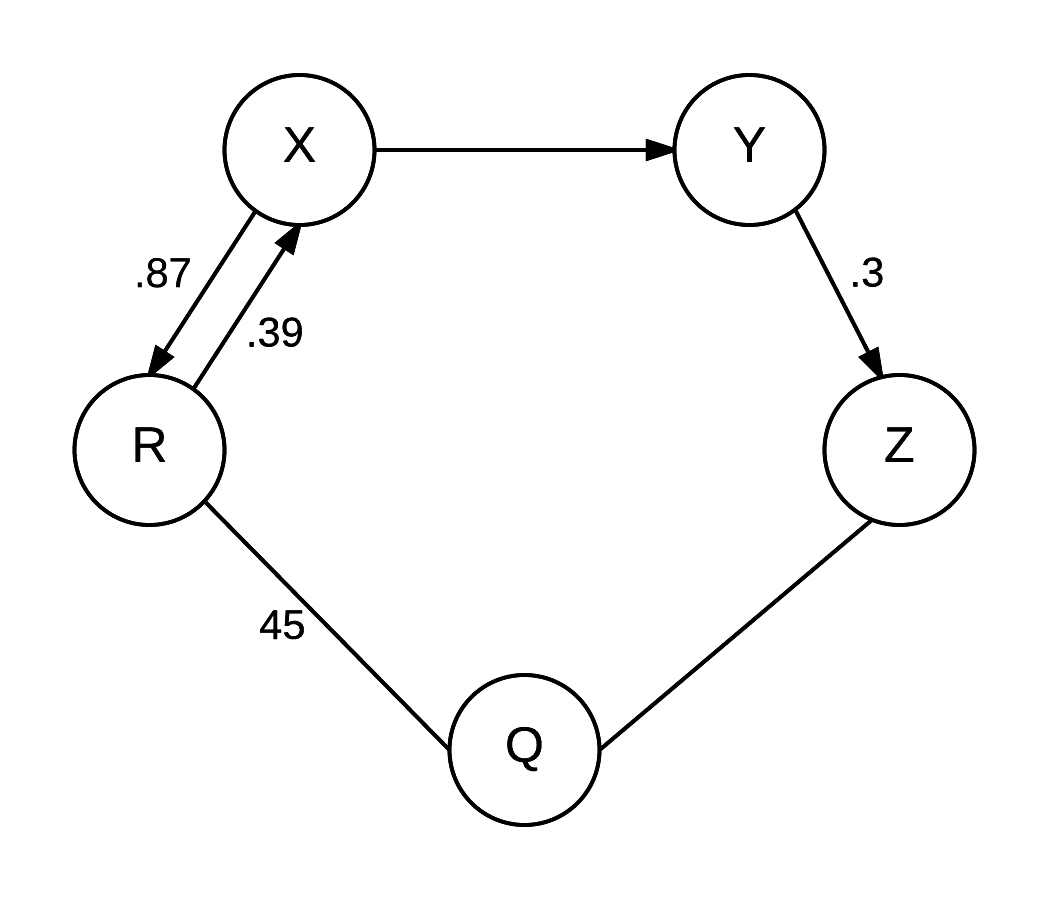
\includegraphics{graphs/node_operators_example.png}
\caption{Example Graph showing nodes with different weights and edges.}
\label{fig:node-ops}
\end{figure}


\begin{lstlisting}[language=pltLang, caption=Shows the use of node operators that creates the graph in Figure \ref{fig:node_ops}., label=lst:node-ops]
node X, Y, Z, Q, R;

X --> Y;
Y -->[.3] Z;
Z -- Q;
Q --[45] R;
R [.87]--[.39] X;

R == Q;    # returns false
R != Q;   # returns true

\* accessing edge lists: *\
X.out[Y]; # == null
Y.out[Z]; # == .3
R.in[X]; # == .87

node alt = Z;
Y.out[alt] == Y.out[Z]; # returns true

\* Alternate Graph Creation:
 * adds the nodes to the graph G, while
 * at the same time it adds edges and weights
 * between the nodes
 *\
node x, y, z, q, r;
graph G = {
    x --> y,
    y -->[.3] z,
    z -- q,
    q --[45] r,
    r [.87]--[.39] x
};
    

\end{lstlisting}

\subsection{Graph Operators}
Hosanna's got this one.


\section{Statements}

\subsection{Expression Statements}
In \pltlang\ expression statements are terminated by a semicolon, and are executed in the order they are read in from top to bottom. All effects from an expression statement are completed before the next one is executed.

\begin{lstlisting}[language=pltLang, label=lst:expression-statements]
\* Examples *\
node y("Hello world"); \* declaration of a node with data "Hello World" *\
num a = 5; \* declaration of number a which equals 5 *\
a = (3 + 3) / 2; \* basic arithmetic, sets a to 3 *\
print(a); \* function call, prints 3 because previous expression executed. *\

\end{lstlisting}

\subsection{Control Flow Statements}
\code{if / else if* / else} and \code{if} conditional statements are supported, where \code{*} represents the Kleene star operator.

\begin{lstlisting}[language=pltLang, label=lst:if-else]
if condition {
  \* execute when condition is true *\
}
else {
  \* if condition is false go here *\
}

if condition {
  \* execute when condition is true *\
}
else if another_condition {
  \* if anothe_condition is true go here *\
}
else if yet_another_condition {
  \* only reached if another_condition is false
  go here if yet_another_condition is true *\
}
else {
  \* execute when all conditions are false *\
}

if condition {
  \* execute if condition is true *\
}
\* continue executing subsequent expression statements *\

\end{lstlisting}

\subsection{Loop Statements}
\pltlang\ supports \code{while} and \code{for} loops.

\subsubsection{While Loops}

\code{while} statements execute repeatedly the code in the scoped block (delimited by braces following the Boolean expression), while the Boolean expression \code{condition} evaluates to true. 

\begin{lstlisting}[language=pltLang, label=lst:while-loop]
while condition {
  \* code *\
}

\end{lstlisting}

\subsubsection{For Loops}
\code{for} statements iterate through all elements in \code{iterable\_var}, assigning the current element to \code{var\_name}. 

\begin{lstlisting}[language=pltLang, label=lst:for-loop]
for var_name in iterable_var {
  \* code *\
}

\* common usage examples *\
for node_var in graph_var {
  \* do something with each node *\
}

for edge_var in n.out {
  \* do something with each outbound edge from node n *\
}

\end{lstlisting}

\subsection{Other Statements}

\subsubsection{Break}
Used in a loop to exit out of the loop immediately. Continue executing expressions after the loop block as expected.

\begin{lstlisting}[language=pltlang, label=lst:break-statement]
num i = 0;
while i < 5 {
  i = i + 1;
  if i == 3 {
    break;
  }
  print(i, ' ');
}
\* Prints 1 2 *\

print(i, ' ');
\* Prints 2 *\

\end{lstlisting}

\subsubsection{Continue}
Used in a loop to skip the rest of the loop block and execute the next iteration of the loop.

\begin{lstlisting}[language=pltLang, label=lst:continue-statement]
num i = 0;
while i < 5 {
  i = i + 1;
  if i == 2 {
    continue;
  }
  print(i, ' ');
}
\* Prints 1 3 4 5 *\

\end{lstlisting}

\subsubsection{Return}
Used to exit from a function and dictate the output argument. The output argument must be the same type as specified in the function header. If not, the compiler will throw an error.

\begin{lstlisting}[language=pltLang, label=lst:return-statement]
def num foo(num n) {
  if n > 2 {
    return 2;
  }
  return 1;
} 

num out1 = foo(10)
print(out1);
\* Prints 2 *\

num out2 = foo(1)
print(out2);
\* Prints 1 *\
\end{lstlisting}


\section{Functions}

\subsection{Function Declaration and Definition}

Before a function can be used, it must be declared and defined. Functions are declared using the \code{def} keyword, followed by the data type the function will return, followed by the function name, followed by a list of parameters enclosed in parentheses. The function must then be immediately defined within a set of curly braces immediately follwing the parentheses of the parameter list. 

\begin{lstlisting}[language=pltLang, caption=Function declaration and definition., label=lst:funct-def]
\* 
 * Outline of function declaration and definition.
 * ``return_type'' would be a data type.
 *\
def return_type function_name () {
  \* function implementation code *\
}
\end{lstlisting}

\subsection{Return Statements}

Each function must return a value that matches the declared return type using the \code{return} keyword. For functions with the \code{null} return type, indicating that nothing is returned by the function, the return statement can consist either of the keyword \code{return} as an expression by itself (line 2 of Listing \ref{lst:funct-return}), or it can explcitly \code{return null} (line 6 of Listing \ref{lst:funct-return}).

\begin{lstlisting}[language=pltLang, caption=Return statements of functions., label=lst:funct-return]
def null fnull1 () {
  return;
}

def null fnull2 () {
  return null;
}

def int fint () {
  return 4;
}
\end{lstlisting}

\subsection{Parameter List}

The declaration of a function must include a list of required parameters enclosed within parentheses. To define a function which requires no parameters, the contents of the parentheses can be left blank. Otherwise, each parameter requires the data type, followed by a variable name by which the parameter can be referenced within the function definition. 

\begin{lstlisting}[language=pltLang, caption=Parameters in function declarations., label=lst:funct-params]
def null no_params () {
  return;
}

def num one_param (num x) {
  num b = x;
  return b;
}

def string multi_params (string s1, num y, string s2) {
  string statement = s1 + " " + " " + y + "s2";
  return statement;
}

\end{lstlisting}

\subsection{Calling Functions}

The syntax for calling a function is: the name of the function, followed by a comma-separated list of values or variables to be used in paremter list enclosed within parentheses. Each value or variable passed in to a function call is mapped to the corresponding variable in the declared parameter list of the function.

A function-call expression is considered of the same type as its return type. Because of this, function-call expressions may be used as any other expression. For example a function-call expression can be used in the assignment of variables, as in line 11 of Listing \ref{lst:funct-call}.

\begin{lstlisting}[language=pltLang, caption=Function declaration and definition., label=lst:funct-call]
def num increment (num n, num incr) {
  return n + incr;
}

num x = 4;

\* The following call maps ``x'' to the variable ``n'',
 * and ``2'' to the variable ``incr'' from the declaration
 * of the ``increment'' function 
 *\
num y = increment(x, 2);

print("y: ", y); # prints --> ``y: 6''
\end{lstlisting}

\subsection{Variable Length Parameter Lists}

The \emph{only} function in \pltlang\ that can have a variable number of parameters is the built-in \code{print} function. All other functions must be declared with a defined absolute number of 0 or more parameters. 

The \code{print} function may be called using a comma-separated list of expressions which can be evaluated as or converted to the \code{string} type. Each of the built-in types may be used directly as an argument to the print function.

\begin{lstlisting}[language=pltLang, caption=The built-in ``print'' function., label=lst:funct-print]
string alpha = "World";
print("Hello", alpha, "\n");

node x("foo");
num n = 20;
print("The node <", x, "> has an associated num equal to:", n, "\n");
\end{lstlisting}

In Listing \ref{lst:funct-print}, the \code{print} function was called on line 2 with 3 arguments and with 5 arguments on line 6. The number of arguments passed to \code{print} does not matter. 

\section{Program Structure and Scope}

\subsection{Program Structure}

A \pltlang\ program consists of a series of function declarations and expressions. Because \pltlang\ is a scripting language, there is no \code{main} function. Instead, expressions are executed in order from top to bottom. Functions must be declared and defined before use. 

\subsection{Scope}

In \pltlang\, variables declared in expressions not belonging to functions or \code{for} loops have scope outside of function definitions. Variables declared in a function are visible or available to be referenced by name within the body of the function (functional scoping). Variables declared in \code{for} loop expressions can be referenced by name within the loop body (lexical scoping). There is no true global scoping as programs are executed from top to bottom. Variable declarations within functions and \code{for} loops can mask variables declared outside.

\begin{lstlisting}[language=pltLang, caption=Example of masking, label=lst:scope-masking]
node n("Hello world");
node x("Goodbye world");
node y("cool");

Graph nodes = {
  x,
  y
};

for node n in nodes {
  print(n, " ya ya ya\n");
}
\* prints
  Goodbye world ya ya ya
  cool ya ya ya*\

print(n);
\* prints Hello world *\
\end{lstlisting}

In Listing \ref{lst:scope-masking}, the declaration of \code{n} in the loop scope masks the declaration of \code{n} from the top level scope.

\section{Sample Program}

\end{document}
